\documentclass{article}

\usepackage[inline]{enumitem}
\usepackage{amsmath}
\usepackage{graphicx}

\newcommand{\ds}{\displaystyle}

\begin{document}

\noindent{}\rule{\textwidth}{0.4pt}
\begin{center}
	Universidade Federal da Grande Dourados\\
	An\'alise Num\'erica --- Lista 5 \\
	Engenharia Mec\^anica --- 2016.2 \\
	Prof.\ Adriano Barbosa
\end{center}
\noindent{}\rule{\textwidth}{0.4pt}

\begin{enumerate}
	\item Calcule a spline c\'ubica natural utilizando os dados abaixo:
		\begin{enumerate}
			\item $(8.3, 17.56492), (8.6, 18.50515)$
			\item $(-0.5, -0.02475), (-0.25, 0.3349375), (0, 1.101)$
		\end{enumerate}

	\item Os dados no exerc\'{\i}cio anterior foram gerados a partir das fun\c{c}\~oes
		abaixo. Use as splines c\'ubicas calculadas para aproximar os valores de
		$f(x)$ e $f'(x)$ e calcule o erro.
		\begin{enumerate}
			\item $f(x) = x \ln(x)$, aproxime $f(8.4)$ e $f'(8.4)$
			\item $f(x) = x^3 + 4.001x^2 + 4.002x + 1.101$, aproxime
				$f\left(-\frac{1}{3}\right)$ e $f'\left(-\frac{1}{3}\right)$
		\end{enumerate}

	% \item Calcule a spline c\'ubica amarrada utilizando os dados abaixo:
	% 	\begin{enumerate}
	% 		\item $(-0.25, 1.33203), (0.25, 0.800781)$
	% 		\item $(0.1, -0.29004996), (0.2, -0.56079734), (0.3, -0.81401972)$
	% 	\end{enumerate}

	% \item Os dados no exerc\'{\i}cio anterior foram gerados a partir das fun\c{c}\~oes
	% 	abaixo. Use as splines c\'ubicas calculadas para aproximar os valores de
	% 	$f(x)$ e $f'(x)$ e calcule o erro.
	% 	\begin{enumerate}
	% 		\item $f(x) = x^4 - x^3 + x^2 - x + 1$, aproxime $f(0)$ e $f'(0)$
	% 		\item $f(x) = x^2 \cos(x) - 3x$, aproxime $f(0.18)$ e $f'(0.18)$
	% 	\end{enumerate}

	\item A spline c\'ubica natural $s$ abaixo est\'a definida em $[0,2]$
		\[s(x) = \left\{\begin{array}{ll}
					s_0(x) = 1+2x-x^3, & \text{se}\ 0 \le x \le 1 \\
					s_1(x) = 2+b(x-1)+c(x-1)^2+d(x-1)^3, & \text{se}\ 1 \le x \le 2
				\end{array}\right.\]
		Encontre $b$, $c$ e $d$.

	\item Calcule a spline c\'ubica natural para aproximar $f(x) = \cos(\pi x)$
		usando os seguintes valores $x=0, 0.25, 0.5, 0.75, 1$. Integre a spline
		no intervalo $[0,1]$ e compare com o valor real da integral
		$\int_0^1\cos(\pi x)\ dx$. Use as derivadas da spline para aproximar
		$f'(0.5)$ e $f''(0.5)$ e compare as aproxima\c{c}\~oes com os valores reais.

	\item Sejas $f$ definida em $[a,b]$ e $a=x_0<x_1<x_2=b$. Mostre que a
		spline quadr\'atica interpolante para o problema acima gera cinco
		equa\c{c}\~oes e seis inc\'ognitas. A condi\c{c}\~ao $s\in C^2[x_0, x_2]$ resolve o
		problema?
\end{enumerate}

Respostas:

As splines abaixo est\~ao escritas na forma:

$s_i(x) = a_i + b_i(x-x_i) c_i{(x-x_i)}^2 + d_i{(x-x_i)}^3,\ \text{para}\
x\in[x_i, x_{i+1}]$

\noindent{}1. (a)

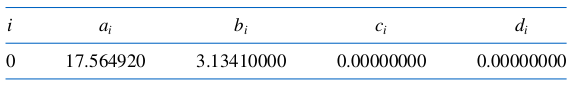
\includegraphics[width=0.75\textwidth]{1a.png}
\newpage{}

(b)

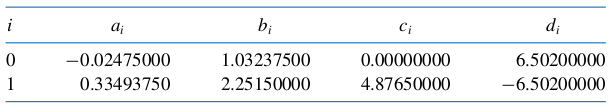
\includegraphics[width=0.75\textwidth]{1b.png}

\noindent{}2.

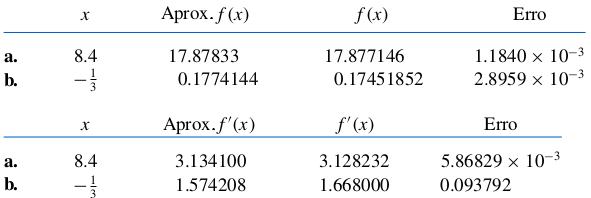
\includegraphics[width=0.75\textwidth]{2.png}

\noindent{}3. $b=-1, c=-3, d=1$

\noindent{}4.

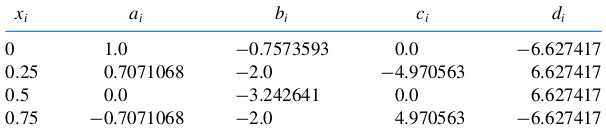
\includegraphics[width=0.75\textwidth]{6.png}
\end{document}  % chktex 16
